\chapter{Sprint 2}
\label{chap:sprint2}
The following section presents an overview of how we planned, worked and
completed sprint two.

Sprint two started on 17th of September and ended on 30th of September.

The chapter is divided into five parts, starting with the overall plan for the
sprint in Section \ref{sec:sprint2sprintplan}. Followed by the sprint backlog, which
enlists the tasks that have been chosen for the sprint. Section
\ref{sec:sprint2designAndImplementation}.
will focus on the work made to the GUI, the logic implemented in the applications 
and the work done to the database and database access in the applications.
The chapter ends with what have been tested and the corresponding results in
Section \ref{sec:sprint2testingAndResults} and a sprint review in Section
\ref{sec:sprint2sprintRetrospective}.

\section{Sprint Plan}
\label{sec:sprint2sprintplan}
The plan for the sprint was to add more of the graphical user interface to the applications.
The GUI implemented during this sprint, would later on be connected to logic to complete the functionality wanted.


We also wanted to add some functionality through adding logic to the different elements of the applications. The main focus was the log, the medication plan, the notifications and the distraction during a treatment. 


We made a change to the sprint plan during the sprint. The problem was that we
had focused too much on hardcoded ``dummy" data, and needed the connection towards
the database working. This lead to a delay on the log, as this part was most
dependent of a working database connection.


\section{Sprint backlog}
This section contains a table with the sprint backlog, which is a smaller part of the product 
backlog. The goal is to implement the entire sprint backlog during the sprint.

\begin{table}[t]
	\begin{center}
		\begin{tabular}{|p{2.0cm}| p{8.0cm}| p{2.0cm}|p{2.0cm}|p{2.0cm}|}
			\hline
			\#  ID 	& Task 	& Story points 	& Estimated hours & Responsible \\
			\hline
			1.1 & Make some kind of distraction through the Karotz		&  8  & 40  & Yngve \\
			\hline
			1.2 & Make method for saving a treatment throught Karotz  	&  4  & 20	& Yngve\\
			\hline
			1.3 & Make method for starting treatment through Karotz  	&  2  & 10	& Yngve\\
			\hline
			1.4 & Make the distraction logic class 						& 10  & 50  & Eirik \\
			\hline
			2.1 & Calendar view for log 								& 10  & 50  & Esben\\
			\hline
			2.2 & Backend solution for saving the log 					& 10  & 50  & \\
			\hline
			3.1 & Make the reminder for Android platform 				&  6  & 30  & Aleksander \\
			\hline
			3.2 & Make the reminder for Karotz 							&  6  & 30  & Yngve \\
			\hline
			3.3 & User interface for changing reminder preferences 		&  6  & 30  & Eirik \\
			\hline
			3.4 & Secure that the reminder is giving independently of 
				  internet connection and sound level on the phone 		&  2  & 10  &  \\
			\hline
			\bfseries{SUM} &											& \bfseries{64} & \bfseries{320} & \\
			\hline
			\hline
		\end{tabular}
	\end{center}
	\caption{Backlog for sprint 2}
\end{table}

We also decided to continously write on the report, attend lectures and hold advisor and 
customer meetings during the sprint. These tasks are not included in the backlog, but the hours 
spent are included in the status reports.

\section{Design and Implementation}
\label{sec:sprint2designAndImplementation}
We continued to add graphical user interface elements to represent the different functionality
in the applications. During this sprint the focus was fairly broad.
The reason for this was the customer's priorities of what functionality should
be implemented, and also that many of the tasks were dependent of each other, and therefore could not be worked on at the same time.

Both we and the customer were also very curious to how the Karotz would
be implemented with the applications. We chose to have one developer focus on this task
during this sprint.

\subsection{User Interface Layer}
We implemented the log as a calendar view. This was based on open source code, 
which we modified, to ensure it would have the properties we wante. At that time, there was still some work that needed to be done to the log. However, it was 
very hard to do these changes until a backend solution was working, so the rest of this 
task was being halted until we had the backend system up and running.

During the sprint we added a basic animation to the distraction, simply counting from zero
to ten, to assure that the animation-logic was in place, and the counting because the child should take ten
breaths from the inhaler during the treatment. After the treatment is finished the user will be rewarded with stars.

To the settings menu we added very simple functionality for making a
treatment plan. By using simple menus a user would be able to choose which medicines should be
included and what dosage of each medicine. The user should also be able to set the time
for reminders. The GUI for this was implemented during the sprint, but the logic and database
connections were yet to be implemented.

We added functionality for dressing up the avatar with different costumes.
At that time the costumes were not changable in the GUI, since the shop was
yet to be implemented.

To the treatment and distraction part of the applications, we implemented logic to make
the treatment understandable for children. We chose to solve this task by using logic to change the GUI.

During the sprint we implemented notifications to remind the user to take his/her medicine.
The logic behind this is done by a "Notification Manager" which fires a method for putting a notification
on the status bar of the phone.

We found out halfway during this sprint that it was necessary to change the notifications into
alarms. Alarms are able to run independently of any other methods, in difference to notifications which
are fired by a method internally. To ensure that the user would get the correct reminders it was
necessary to change this.


\subsection{Data Persistence Layer}
The development team found a severe problem with the current database server.
The problem is that we cannot access the database unless a client (android
device) is connected to NTNU's network. The customer unsuccessfully worked on trying to find another server we could use, therefore we had to change the
architecture, and make a seperate application on one of our
``folk.ntnu.no''-domains, and access the database from this webservice. 

We were in a stage where we needed some test-data to see any progress, so we
continued to load the database with somewhat relevant testing data.

\subsection{Database Access Layer}
During the sprint, it was discovered that the Karotz cannot directly access the database, and that the
NTNU MySQL server cannot be accessed from outside the school network. These two problems lead to the
creation of an additional layer to access the database.

The \emph{Database Access Layer} is a set of PHP web pages currently hosted at \url{http://folk.ntnu.no/yngvesva/blopp}
designed to take input in the form of GET and POST parameters, access the database and either get
information from or modify it, and return data in JSON format. This layer is further described
in section \ref{sec:databaseAccessLayer}.

The additional work created by the tasks related to the database access layer meant that there was
substantially more work to be done in the sprint than was planned before it started.

The modules created this sprint were:
\begin{itemize}
  \item \emph{add\_child.php:} Takes a name, personal number (SSN) and a list of states (integer IDs) that the child can have. Creates an entry in the \code{CHILDREN} table for the child, an avatar entry and a medical plan entry. Also creates an entry in \code{CHILD\_HEALTH\_STATES} for all the states the child can have. Returns the generated \code{avatar\_id} and \code{medical\_plan\_id}.
  \item \emph{get\_available\_child\_states.php:} Takes a child \code{ID} and returns a list of the labels (colors, names) and IDs of the states the child can have.
  \item \emph{get\_child.php:} Takes an ID of a child and returns all the columns for the given ID in the \code{CHILDREN} table.
  \item \emph{get\_child\_state.php:} Accepts a child ID and returns the ID and label of the current state of the child.
  \item \emph{get\_doses\_for\_current\_state.php:} Takes a child ID and returns a list of planned doses of medicines for that day. The fields of each entry are: \code{id}, \code{medical\_plan\_id}, \code{health\_state\_id}, \code{time}, \code{medicine\_id}, \code{medicine\_karotz\_color} and \code{medicine\_name}.
  \item \emph{register\_medicine\_taken.php:} Register a dose of medicine taken. Accepts a post object with the fields \code{child\_id}, \code{medicine\_id}, \code{time}, \code{day\_date}, \code{health\_state\_id} and \code{medical\_plan\_dose\_id}. If there is an entry for that dose id that day, the method does nothing and simply returns $unique=false$. Otherwise, it calculates a reward, and updates \code{DAY\_MEDICINE\_DOSES} with the entry. Returns the reward for that dose.
  \item \emph{set\_child\_state.php:} Takes a child ID and a state ID and sets the current state of the given child to that one.
\end{itemize}

\section{Testing and Results}
\label{sec:sprint2testingAndResults}

\subsection{Testing}
The testing done during this sprint was mainly concerned with the backend logic of the system,
since the basic graphical layout functionallity was tested during the previous sprint. We did 
testing on the database-connection and 
the sql-queries, aswell as the repositories we created for the client side of the system.

\begin{table}
	\begin{center}
		\begin{tabular}{|p{3.0cm}|p{14.0cm}|}
			\hline
			\bf{Item} & \bf{Description}\\
			\hline
			\bf{ID} & UNIT2.1\\
			\bf{Description} & Test of the distraction sequence\\
			\bf{Date} & 30.09.2012\\
			\bf{Responsible} & Eirik\\
			\bf{Subject} & \code{Distraction} and \code{DistractionActivity} classes in \code{no.blopp.app.med.activities} package\\
			\bf{Precondition} & Working version of CAPP, runable on the android virtual device\\
			\bf{Steps} &
			\begin{tabulenum}
			  \item Press "Start Treatment" on the \code{MainMenu}.
			  \item Press the next-button on the screen, after seeing that the avatar is updated, and it shows the right medicine.
			  \item Watch the animation, press the next-button.
			  \item Press the shop button or the main menu button to navigate away from the finish-screen.
			\end{tabulenum}\\
			\hline
			\bf{Results} & Application updated the avatar correctly. Pressing the next-button while the animation was still running caused the application to crash.\\
			\hline
		\end{tabular}
	\end{center}
	\caption{Unit test 2.1, CAPP distraction sequence}
	\label{tab:unit2.1}
\end{table}

\begin{table}
	\begin{center}
		\begin{tabular}{|p{3.0cm}|p{14.0cm}|}
			\hline
			\bf{Item} & \bf{Description}\\
			\hline
			\bf{ID} & UNIT2.2\\
			\bf{Description} & Test of database connection\\
			\bf{Date} & 26.09.2012\\
			\bf{Responsible} & Esben\\
			\bf{Subject} & \code{DBConnection}\\
			\bf{Precondition} & ---\\
			\bf{Steps} &
			
				Unit test of \code{DBConnection.java}. Run the application as Java Application \\
			\hline
			\bf{Results} & 
			\begin{tabulenum}
			  \item If connected to NTNU's network via VPN (virtual private network): Connection succeeded.
			  \item If not connected to NTNU's network: Connection failed
			\end{tabulenum}\\
			\hline
		\end{tabular}
	\end{center}
	\caption{Unit test 2.2, database connection}
	\label{tab:unit2.2}
\end{table}

\begin{table}
	\begin{center}
		\begin{tabular}{|p{3.0cm}|p{14.0cm}|}
			\hline
			\bf{Item} & \bf{Description}\\
			\hline
			\bf{ID} & UNIT2.3\\
			\bf{Description} & Testing of SQL-queries\\
			\bf{Date} & 30.09.2012\\
			\bf{Responsible} & Esben\\
			\bf{Subject} & \code{LogModelRepository}\\
			\bf{Precondition} & Connected to NTNU's network\\
			\bf{Steps} &
			
				Unit test of \code{LogModelRepository.java}. Run the application as Java Application\\ 
			\hline
			\bf{Results} & 
			Success. The fields asked for were the same as stored in the database.\\
			\hline
		\end{tabular}
	\end{center}
	\caption{Unit test 2.3, SQL queries}
	\label{tab:unit2.3}
\end{table}

\subsection{Results}
We see that there is a big problem with using NTNU's MySQL server since it cannot be accessed
from points external to the NTNU subnet. This problem is currently being discussed by the 
customer, and we might, get access to a server that is not dependent on the network the unit 
is at. Other than that, no major errors were found.

\section{Sprint Retrospective}
\label{sec:sprint2sprintRetrospective}
This section contains an evaluation of the Sprint. The evaluation is done mainly
by the developer team, but feedback from the customers were added to the
retrospect.

\subsection*{What went well?}
Our programming event held thursday 20th of September was a great success. The
group works much better when we're working physically together. We feel that we
have a good code base, and can start building the applications more efficiently
during the upcoming sprints. 

\subsection*{What shall we start doing?}
We identified four elements that should be added to our sprints:
\begin{enumerate}
  \item Be more accurate towards deadlines with the customer.
  \item Make better conventions for naming of fields in the source code.
  \item Make better sprint plans to reflect the need of the backend system.
  \item We need a predetermined day to write the reports for each sprint. 
\end{enumerate}

\subsection*{What could have gone better?}
We must learn to send the meeting reports to the customer within 24 hours. We
should have communicated better on who was going to send the report after J\o rgen
drowned his computer after a customer meeting. 


\subsection*{What should we stop doing?}
Naming fields (buttons, textviews etc. from the Android framework) inconsistently
with the conventions stated in section \ref{chap:codingTemplates}

\begin{table}[t]
	\centering
	\begin{sideways}
		\begin{tabular}{|l | p{6.5cm} | c | c | c | c | l |}
			\hline
			  \#  ID 	& Task 	& Story points 	& Estimated & Actual &
			  Estimated Left & Responsible \\
			\hline
			  1.1 & Make some kind of distraction through Karotz 		& 8  	& 40	&  18 & 10
			  & Yngve
			  \\
			\hline
			  1.2 & Make method for saving a treatment through Karotz  	& 4  	& 20 & -- & 20 &
			  --
			  \\
			\hline
			  1.3 & Make method for starting treatment through Karotz 	& 2	&   	10	& 9 & 4 &
			  Yngve \\
			\hline
			  1.4 & Make the distraction logic class 							& 10  & 50 & 41 & 0 & Eirik \\
			\hline
			  2.1 & Calendar view for log & 10 & 50 & 20 & 15 &  Esben \\
			\hline
			2.2 & Backend solution for saving the log & 10 & 50 & 4 & 45 & Esben \\
			\hline
			3.1 & Create GUI for settings & 1 & 5 & 1 & 0 & Jørgen  \\
			\hline
			3.2 & Create navigation for settings & 1 & 5 & 3 & 0 & Jørgen  \\
			\hline
			4.1 & Make the reminder for Android Platform & 6 & 30 & 14 & 20 & Aleksander \\
			\hline
			4.2 & Make the reminder for Karotz & 6 & 30 & 7 & 24 & Yngve \\
			\hline
			4.3 & User interface for changing reminder preferences & 6 & 30 & 0 & 30 & -- \\
			\hline
			4.4 & Secure that the reminder is giving independently of internet connection and sound level on the phone
			 & 2 & 10 & 1.5 & 10 & Aleksander \\
			\hline
			5.1 & Make database access layer & 3 & 15 & 14 & 20 & Yngve \\
			\hline
			5.2 & Make repositories & 10 & 50 & 4 & 45 & Esben \\
			\hline
			\bfseries{SUM} & & \bfseries{64} & \bfseries{320} & \bfseries{136.5} & \bfseries{243} & \\
			\hline
			\hline
		\end{tabular}
	\end{sideways}
	\caption{Sprint burndown chart, Sprint 2}
	\label{tab:sprint2burndown}
\end{table}

\begin{figure}[t]
	\begin{center}
		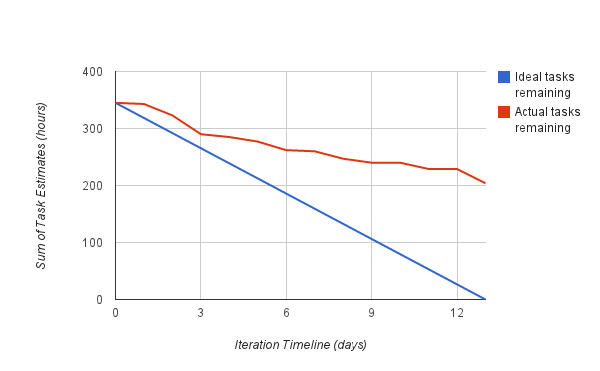
\includegraphics[width=15cm]{Pictures/Charts/Sprint2burndown}
	\end{center}
	\caption{Sprint 2 burndown chart}
	\label{fig:sprint2burndown}
\end{figure}

\subsection{Sprint Burndown Chart}
Figure \ref{fig:sprint2burndown} and Table \ref{tab:sprint2burndown} show the burndown chart for the second sprint. At first glimpse the sprint burndown chart doesn't look too good. We started of at a farily good pace. 
At Thursday 20th of September we held a fellow programming session, which was very successful. This resulted 
in a small dent in the chart, in the positive direction. During the second week of the sprint, we had 
some difficulties. First off, one of us had to step down on working hours, due to illness in his 
family. Second, the other team members had assignments to finish in other courses. This stole much of the 
time which was supposed to be used on programming.

Also, during the sprint the developers discovered problems technical problems the could not foresee in advance. 
The database is hosted on a NTNU-server, resulting in the need of VPN-connection to work outside of the university's 
internet network. We, in agreement with the customer, decided to make a web service to handle the traffic 
to the database. This resulted in an increase in story points for the task.

Our goal for each two-week sprint is to finish 175 estimated work hours, which with a base multiplier of 5 correlates to
$175/5=35$ story points. The backlog contained 64 story points in total, so we had no ambition of completing all the tasks.
However, at the end of the sprint there were 243 estimated work hours left, which corresponds to $243/5=48.6$ story points.
In other words, we only completed $64-48.6=15.4$ story points in the second sprint. This is less than half of the amount we
wanted to complete. We were not satisfied with the progress, and understands we need to step up the amount of work done in 
the upcoming sprints, in order to finish the prototype.
\clearpage{}
\blankpage{}